\appendix

\chapter{Appendix}

\section{Relationship between \acl{MAC} Operations and the Number of Parameters}\label{sec:appendix:macs}

For a convolution operation, the number of parameters of a layer is not
representative of its computational complexity. Each kernel has to be spatially
convolved with the entire input. The resulting convolutional complexity is, for
one part, highly dependent on the input size, and for the other part, higher
than the number of parameters.\\

Without loss of generality, consider a 2D square matrix $M$ of size $m \times
m$, and a 2D convolution kernel $K$ of size $k \times k$, with $k<m$. The output
of the spatial convolution of $M$ by $K$ is denoted $O$. The matrix $O$ is of
size $(m-k+1) \times (m-k+1)$. Each one of the $(m-k+1)^2$ elements of $O$
necessitates $k^2$ multiplications and $k^2-1$ additions. For the sake of
simplicity, we will consider $k^2$ \acfp{MAC} operations per element of $O$. The
total number of \acp{MAC} needed to compute $O$, denoted $\mu$, is therefore:\\
$$
\mu = (m-k+1)^2 \times k^2
$$\\

Considering that there are $k^2$ elements in $K$, the ratio between the number
of \acp{MAC} and the number of parameters is:

$$
\frac{\mu}{k^2} = (m-k+1)^2
$$\\


Since $k<m$, the ratio $\frac{\mu}{k^2}$ is always greater than $1$, and grows
quadratically with $m$. Therefore, for a 2D convolution, the computational
complexity can roughly be estimated as $(m-k+1)^2$ times the number of
parameters in the convolution kernel.\\

\section{Annihiliation of the Mixing Coefficient \texorpdfstring{$\lambda$}{lambda}}
\label{sec:appendix:annihilation}

\begin{figure}[!h]
\centering
\subfloat[increasing\label{fig:appendix:annihilation_increasing}]{
    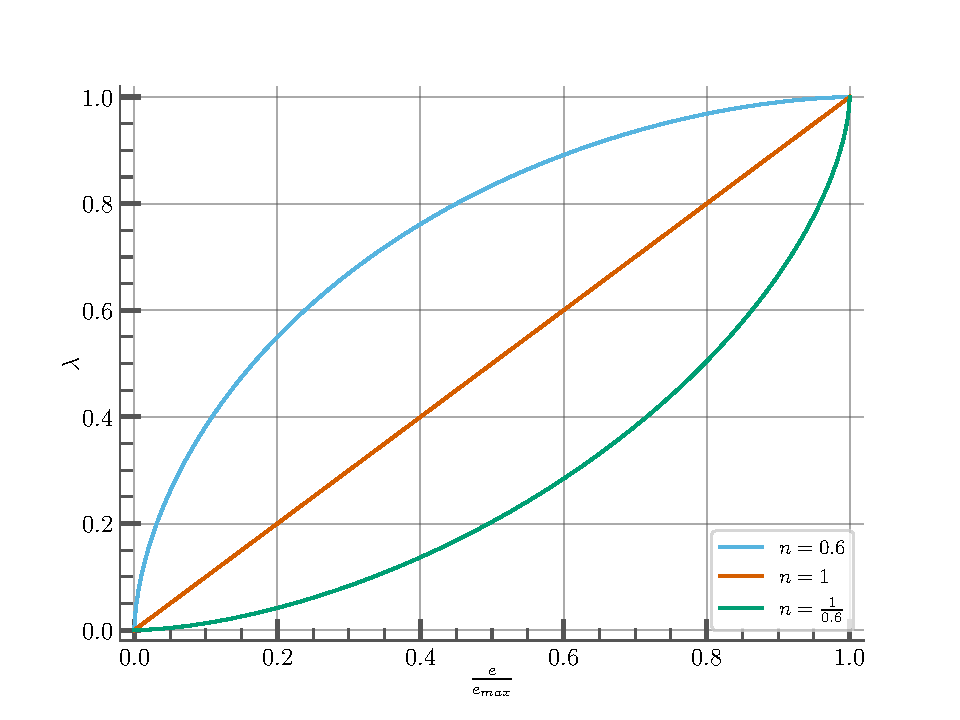
\includegraphics[width=0.49\textwidth]{appendix/assets/annihiling_lambda_max.pdf}}
\subfloat[decreasing\label{fig:appendix:annihilation_decreasing}]{
    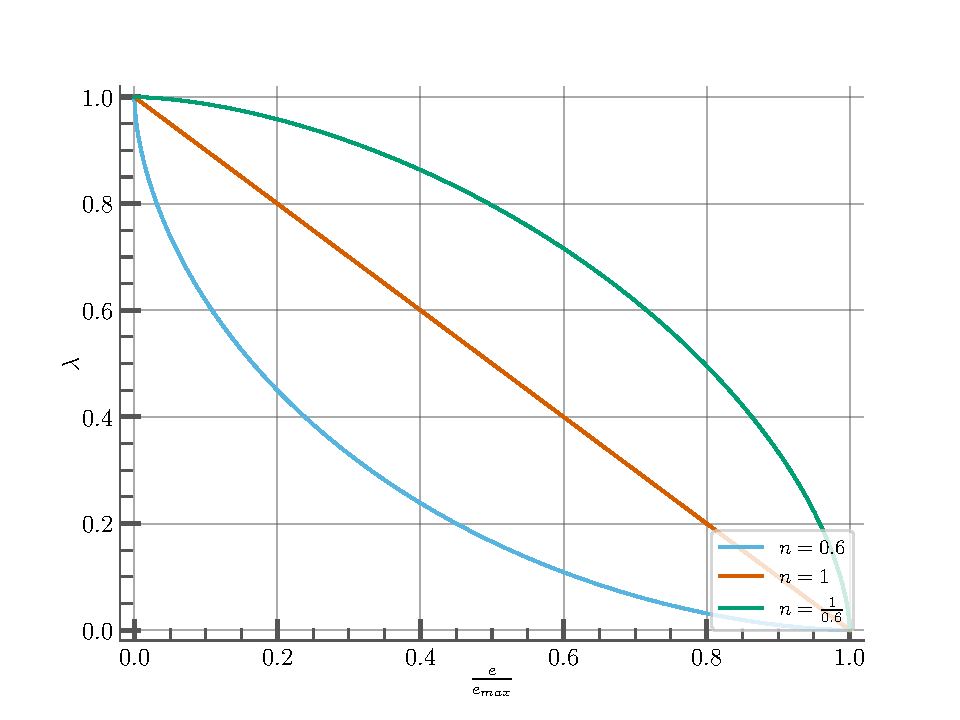
\includegraphics[width=0.49\textwidth]{appendix/assets/annihiling_lambda_min.pdf}}
\end{figure}